\documentclass[11pt]{report}
% Same style as 1-foundations/theory/preamble.tex (the course's own documents).

\usepackage[a4paper,margin=2.3cm,headheight=14pt]{geometry}
\usepackage[T1]{fontenc}
\usepackage[utf8]{inputenc}
\usepackage{lmodern}
\usepackage{microtype}
\usepackage{booktabs}
\usepackage{longtable}
\usepackage{array}
\usepackage{xcolor}
\usepackage{enumitem}
\usepackage{amssymb}
\usepackage{amsmath}
\usepackage{fancyhdr}
\usepackage{listings}
\usepackage{tikz}
\usetikzlibrary{arrows.meta,positioning,calc,fit,shapes.geometric,decorations.pathreplacing}
\usepackage[hidelinks]{hyperref}

\definecolor{warnbg}{RGB}{255,247,230}
\definecolor{warnrule}{RGB}{204,136,0}
\definecolor{newbg}{RGB}{235,245,255}
\definecolor{newrule}{RGB}{40,110,190}
\definecolor{keybg}{RGB}{237,247,237}
\definecolor{keyrule}{RGB}{50,120,60}
\definecolor{headgray}{RGB}{90,90,90}
\definecolor{codebg}{RGB}{248,248,248}

\usepackage[most]{tcolorbox}

\newtcolorbox{warnbox}[1][]{colback=warnbg,colframe=warnrule,boxrule=0.8pt,
  left=6pt,right=6pt,top=5pt,bottom=5pt,arc=1pt,#1}
\newtcolorbox{infobox}[1][]{colback=newbg,colframe=newrule,boxrule=0.8pt,
  left=6pt,right=6pt,top=5pt,bottom=5pt,arc=1pt,#1}
% "In SWEB": where the idea shows up in the course's kernel
\newtcolorbox{swebbox}[1][]{colback=newbg,colframe=newrule,boxrule=0.8pt,
  left=6pt,right=6pt,top=5pt,bottom=5pt,arc=1pt,
  title={In SWEB},fonttitle=\bfseries\small,coltitle=white,colbacktitle=newrule,#1}
% end-of-chapter summary
\newtcolorbox{keybox}[1][]{colback=keybg,colframe=keyrule,boxrule=0.8pt,
  left=6pt,right=6pt,top=5pt,bottom=5pt,arc=1pt,
  title={Key points},fonttitle=\bfseries\small,coltitle=white,colbacktitle=keyrule,#1}

\newcommand{\tbd}{\textcolor{warnrule}{\textbf{[confirm]}}}
\newcommand{\code}[1]{\texttt{#1}}
\newcommand{\file}[1]{\texttt{\small #1}}
\newcommand{\module}[1]{\textsf{module~#1}}

\setlist[itemize]{topsep=2pt,itemsep=1.5pt,parsep=0pt,leftmargin=1.3em}
\setlist[enumerate]{topsep=2pt,itemsep=1.5pt,parsep=0pt,leftmargin=1.6em}
\setlist[description]{topsep=2pt,itemsep=1.5pt,parsep=0pt,leftmargin=1.3em}

\newcolumntype{L}[1]{>{\raggedright\arraybackslash}p{#1}}

\lstset{
  language=C,
  basicstyle=\ttfamily\small,
  keywordstyle=\color{newrule}\bfseries,
  commentstyle=\color{headgray}\itshape,
  stringstyle=\color{warnrule!80!black},
  backgroundcolor=\color{codebg},
  frame=single, rulecolor=\color{black!15}, framesep=3pt,
  xleftmargin=4pt, xrightmargin=4pt, aboveskip=6pt, belowskip=4pt,
  columns=fullflexible, keepspaces=true, showstringspaces=false,
  upquote=true, tabsize=2,
  morekeywords={size_t,ssize_t,pid_t,pthread_t,pthread_mutex_t,pthread_cond_t,
                sem_t,uint8_t,uint32_t,uint64_t,bool,_Atomic,atomic_int,
                atomic_flag,__thread,_Noreturn,__asm__,volatile,pointer,uint64}
}
\lstdefinestyle{shell}{language=bash,morekeywords={},keywordstyle=\color{black}}
\lstdefinestyle{cpp}{language=C++}

\pagestyle{fancy}
\fancyhf{}
\renewcommand{\headrulewidth}{0.4pt}
\fancyhead[L]{\small\textcolor{headgray}{SWEB interview guide}}
\fancyhead[R]{\small\textcolor{headgray}{\leftmark}}
\fancyfoot[C]{\small\thepage}
\renewcommand{\chaptermark}[1]{\markboth{\thechapter\ \ #1}{}}
\fancypagestyle{plain}{\fancyhf{}\renewcommand{\headrulewidth}{0pt}\fancyfoot[C]{\small\thepage}}

\renewcommand{\arraystretch}{1.25}
\setlength{\parskip}{3pt}
\setlength{\parindent}{0pt}
\setlength{\emergencystretch}{3em}   % fewer overfull lines with long \code words

% guide additions
\newtcolorbox{lockbox}[1][]{colback=warnbg,colframe=warnrule,boxrule=0.8pt,
  left=6pt,right=6pt,top=5pt,bottom=5pt,arc=1pt,
  title={Locking},fonttitle=\bfseries\small,coltitle=white,colbacktitle=warnrule,#1}
\newtcolorbox{trapbox}[1][]{colback=warnbg,colframe=warnrule,boxrule=0.8pt,
  left=6pt,right=6pt,top=5pt,bottom=5pt,arc=1pt,
  title={Trap},fonttitle=\bfseries\small,coltitle=white,colbacktitle=warnrule,#1}
\lstset{morekeywords={ScopeLock,Mutex,Condition,SpinLock,ArchThreadRegisters,ArchMemoryMapping},
  breaklines=true, breakatwhitespace=true, postbreak=\mbox{\textcolor{headgray}{$\hookrightarrow$}\space}}
\renewcommand{\file}[1]{\texttt{#1}}   % inherit the size of the surrounding text (tables use \footnotesize)

\renewcommand{\thesection}{\arabic{section}}
\fancyhead[L]{\small\textcolor{headgray}{A1-12 sbrk -- walkthrough}}
\fancyhead[R]{}
\newcommand{\why}[1]{\par\smallskip\noindent\textbf{#1}\par\nopagebreak}
\newcommand{\done}[1]{\begin{keybox}[title={Done when}]#1\end{keybox}}

\begin{document}

{\centering
  {\LARGE\bfseries A1-12 sbrk -- step by step\par}
  \vspace{4pt}
  {\large every line of code, and the theory behind it\par}
  \vspace{8pt}
}

\begin{infobox}
\textbf{How to use this.} Do one step at a time: read it, type the code yourself (do not copy-paste --
typing is how it sticks), check the ``Done when'' box, then go on. Before you start:
\code{task start a1-12}. At the end: \code{task test}, done when \textbf{7 of 7} checks pass and the
last access kills the process.\\[3pt]
\textbf{Theory:} \file{concepts.pdf} \S3 sbrk \& demand paging, \S4 page faults, \S16 page tables.
The same pattern as A0-03 heaplimit -- only the number you store and the syscall differ.
\end{infobox}

\section*{The goal (level 1)}

\begin{lstlisting}[language={},basicstyle=\ttfamily\footnotesize]
Name:         sbrk (POSIX, unistd.h - the stub exists)
Nr:           1700
Description:  Every process has a program break, starting at 0x600000000000.
              sbrk(increment) moves it by increment bytes (may be negative) and returns
              the OLD break. Memory below the break is usable; it is mapped (zeroed) on
              first access by the page fault handler. Shrinking unmaps every page that is
              now completely above the break. An access above the break kills the process.
Return Value: old break, or (void*) -1 if the new break would be below the start or more
              than 4096 pages above it
\end{lstlisting}

\textbf{sbrk} = ``set break''. The \textbf{break} is the end of the heap: everything from the heap
start up to the break may be used, everything above it may not.

\begin{center}
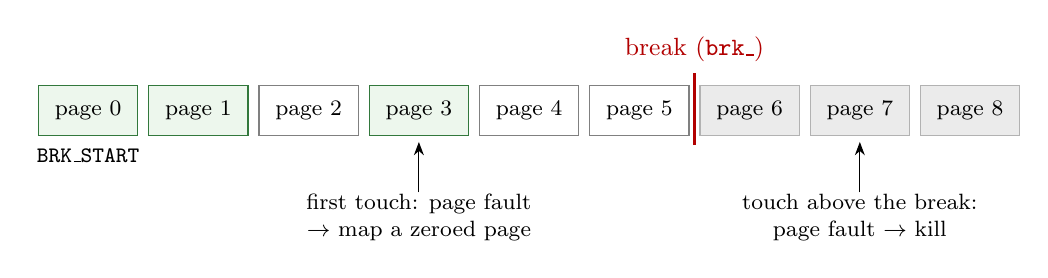
\begin{tikzpicture}[x=1.4cm,y=0.8cm,font=\small]
  \foreach \i in {0,1,3} {\fill[keybg] (\i,0) rectangle +(0.9,0.8); \draw[keyrule] (\i,0) rectangle +(0.9,0.8);}
  \foreach \i in {2,4,5} {\draw[black!50] (\i,0) rectangle +(0.9,0.8);}
  \foreach \i in {6,7,8} {\fill[black!8] (\i,0) rectangle +(0.9,0.8); \draw[black!30] (\i,0) rectangle +(0.9,0.8);}
  \foreach \i in {0,...,8} {\node at (\i+0.45,0.4) {\footnotesize page \i};}
  \draw[very thick,red!70!black] (5.95,-0.15) -- (5.95,1.0) node[above] {break (\code{brk\_})};
  \node[below] at (0.45,-0.05) {\footnotesize \code{BRK\_START}};
  \draw[-{Stealth}] (3.45,-0.9) -- (3.45,-0.1);
  \node[align=center,font=\footnotesize] at (3.45,-1.3) {first touch: page fault\\$\to$ map a zeroed page};
  \draw[-{Stealth}] (7.45,-0.9) -- (7.45,-0.1);
  \node[align=center,font=\footnotesize] at (7.45,-1.3) {touch above the break:\\page fault $\to$ kill};
\end{tikzpicture}

{\footnotesize green = mapped (has RAM) \quad white = below the break, never touched \quad grey = above the break}
\end{center}

Pages are \textbf{not} mapped left to right: the program touches them in any order, and each one gets
RAM at its first touch. All threads of a process share this one heap and this one break.

\section*{The order: 7 steps}

{\small\begin{tabular}{@{}l L{5.2cm} L{4.2cm} L{5.4cm}@{}}
\toprule
\# & What & File & Why in this order\\\midrule
1 & constants + the break variable & \file{UserProcess.h} & first the \textbf{data}: everything else uses it\\
2 & the syscall number & \file{syscall-definitions.h} & user space and kernel must agree on the number\\
3 & the \code{case} & \file{Syscall.cpp} & the kernel's entry point\\
4 & the libc function & \file{unistd.c} & the program's entry point\\
5 & \code{sbrk}: move the break & \file{UserProcess.cpp} & the syscall logic\\
6 & \code{mapBrkPage}: map one page & \file{UserProcess.cpp} & the page fault logic\\
7 & the \code{if} in the handler & \file{PageFaultHandler.cpp} & connects page faults to step 6\\
\bottomrule
\end{tabular}}

\begin{center}
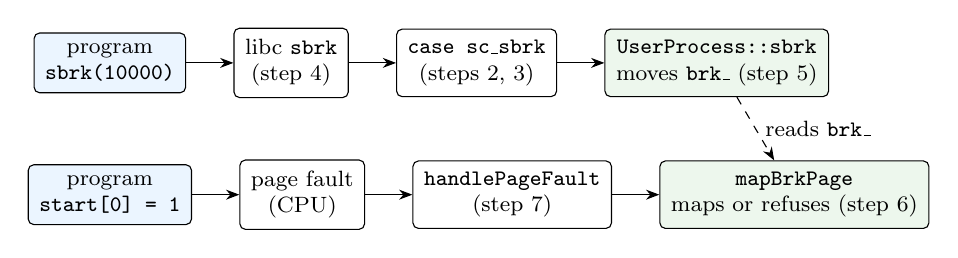
\begin{tikzpicture}[font=\footnotesize, box/.style={draw,rounded corners=2pt,align=center,inner sep=4pt}]
  \node[box,fill=newbg] (prog) {program\\\code{sbrk(10000)}};
  \node[box,right=0.6cm of prog] (libc) {libc \code{sbrk}\\(step 4)};
  \node[box,right=0.6cm of libc] (case) {\code{case sc\_sbrk}\\(steps 2, 3)};
  \node[box,right=0.6cm of case,fill=keybg] (sbrk) {\code{UserProcess::sbrk}\\moves \code{brk\_} (step 5)};
  \draw[-{Stealth}] (prog) -- (libc); \draw[-{Stealth}] (libc) -- (case); \draw[-{Stealth}] (case) -- (sbrk);
  \node[box,below=0.9cm of prog,fill=newbg] (touch) {program\\\code{start[0] = 1}};
  \node[box,right=0.6cm of touch] (pf) {page fault\\(CPU)};
  \node[box,right=0.6cm of pf] (h) {\code{handlePageFault}\\(step 7)};
  \node[box,right=0.6cm of h,fill=keybg] (map) {\code{mapBrkPage}\\maps or refuses (step 6)};
  \draw[-{Stealth}] (touch) -- (pf); \draw[-{Stealth}] (pf) -- (h); \draw[-{Stealth}] (h) -- (map);
  \draw[dashed,-{Stealth}] (sbrk) -- node[right,align=left] {reads \code{brk\_}} (map);
\end{tikzpicture}
\end{center}

% =====================================================================================
\section{The data \hfill {\normalsize\file{common/include/kernel/UserProcess.h}}}

\subsection*{1a: two constants, next to the other \code{\#define}s (after line 19)}

\begin{lstlisting}[style=cpp]
#define BRK_START 0x0000600000000000ULL
#define BRK_MAX (4096 * PAGE_SIZE)
\end{lstlisting}

\why{\code{BRK\_START}: where the heap begins.}
\begin{itemize}
  \item The kernel has to know where the heap is, so it can recognise ``this page fault is a heap access''.
  \item \code{0x600000000000} is far away from the code (at the bottom, around \code{0x400000}) and the
        stacks (at the top, near \code{0x7FFF\ldots}), so the heap can never collide with them.
  \item \code{ULL} = \emph{unsigned long long}. The number is bigger than 32 bits; without \code{ULL} the
        compiler might treat it as a too-small type.
\end{itemize}

\why{\code{BRK\_MAX}: how big the heap may become at most.}
\begin{itemize}
  \item The card says: at most 4096 pages above the start. $4096 \times 4096$ bytes = 16 MiB.
  \item Why a maximum? Without one, a program could move its break into the stack region or up to the
        kernel, and the kernel could not recognise heap addresses clearly.
  \item \textbf{The brackets:} a \code{\#define} is pure text replacement. Without them, \code{x / BRK\_MAX}
        would become \code{x / 4096 * PAGE\_SIZE} -- wrong. Rule: put the whole replacement in brackets.
\end{itemize}

\subsection*{1b: two method declarations, in the \code{public:} part (e.g.\ after \code{cancelThread}, line 172)}

\begin{lstlisting}[style=cpp]
bool mapBrkPage(size_t vpn);
size_t sbrk(ssize_t increment);
\end{lstlisting}

\why{Why in \code{UserProcess}?}
The break belongs to \textbf{one process} and is shared by all its threads, so the methods that use it
belong to that process too. They also need \code{arch\_memory\_} and \code{thread\_lock\_}, which are
private members of \code{UserProcess} -- only its own methods can access them.

\why{\code{mapBrkPage(size\_t vpn)}}
\begin{itemize}
  \item Gets a \textbf{page number} (not an address), because page tables work with page numbers.
  \item Returns \code{bool}: \code{true} = the access was allowed and the page is there;
        \code{false} = it was above the break.
\end{itemize}

\why{\code{sbrk(ssize\_t increment)}}
\begin{itemize}
  \item \code{ssize\_t} (with an s = \textbf{signed}), because the increment can be \textbf{negative}
        (shrinking). \code{size\_t} cannot hold negative numbers: $-4096$ would become a huge positive number.
  \item Returns \code{size\_t}: the old break, which is an address -- or \code{(size\_t) -1} for an error.
\end{itemize}

\subsection*{1c: the break itself, in the \code{private:} part at the very bottom (after \code{threads\_}, line 282)}

\begin{lstlisting}[style=cpp]
size_t brk_ = BRK_START;
\end{lstlisting}

\begin{itemize}
  \item \textbf{The most important variable of the task:} where the heap currently ends.
  \item \code{= BRK\_START}: at the beginning the heap is empty, so its end equals its start. Writing the
        start value directly here means you do not have to change the long constructor.
  \item \textbf{The trailing \code{\_}:} the naming style of the file for members (\code{threads\_},
        \code{running\_threads\_}).
  \item \textbf{Protected by \code{thread\_lock\_}:} whoever reads or writes \code{brk\_} must hold that
        lock. The compiler does not enforce this -- it is a rule you keep yourself.
\end{itemize}

\done{The three parts are in \file{UserProcess.h}. It does not have to compile yet -- the methods do
not exist yet.}

% =====================================================================================
\section{The syscall number \hfill {\normalsize\file{common/include/kernel/syscall-definitions.h}}}

\begin{lstlisting}[style=cpp]
#define sc_sbrk 1700
\end{lstlisting}

\begin{itemize}
  \item A syscall is called \textbf{by number}: the program puts \code{1700} into a register and
        executes the \code{syscall} instruction; the kernel looks at the number to know what is wanted.
  \item This one file is included by \textbf{both} sides -- the kernel (\file{Syscall.cpp}) and the libc
        (\file{unistd.c}) -- so both always agree on the number.
  \item Put it in numeric order next to the others (e.g.\ after \code{sc\_pthread\_detach}).
\end{itemize}

\done{One line added.}

% =====================================================================================
\section{The \code{case} \hfill {\normalsize\file{common/source/kernel/Syscall.cpp}}}

In \code{Syscall::syscallException}, inside the big \code{switch}, e.g.\ after \code{case sc\_execv} (line 92):

\begin{lstlisting}[style=cpp]
case sc_sbrk:
  return_value = currentThread->getProcess()->sbrk((ssize_t) arg1);
  break;
\end{lstlisting}

\begin{itemize}
  \item \code{syscallException} is \textbf{the} entry point of every syscall: the \code{switch} picks the
        function by the number from step 2.
  \item \code{arg1} is the first argument the program passed -- the increment. It arrives as
        \code{size\_t} (registers are just 64 bits, without a sign). The cast \code{(ssize\_t)} reads it
        as signed again, so $-4096$ stays $-4096$.
  \item \code{currentThread->getProcess()}: the process of the thread that made the syscall -- its break
        is the one to move.
  \item \code{return\_value =}: whatever you assign here ends up in the program's \code{rax} register --
        the return value of \code{sbrk} in user space. Forget it, and the program never sees the old break.
  \item No \code{Syscall::sbrk} function and nothing in \file{Syscall.h}: the work goes straight to
        \code{UserProcess::sbrk}, because the break belongs to the process.
\end{itemize}

\done{Three lines in the \code{switch}.}

% =====================================================================================
\section{The libc function \hfill {\normalsize\file{userspace/libc/src/unistd.c}}}

The stub already exists (line 37) and returns \code{(void*) -1}. Replace its body:

\begin{lstlisting}
void* sbrk(intptr_t increment)
{
  return (void*) __syscall(sc_sbrk, (size_t) increment, 0x00, 0x00, 0x00, 0x00);
}
\end{lstlisting}

\begin{itemize}
  \item This is what the program calls. It does nothing itself -- it only \textbf{enters the kernel} with
        the number \code{sc\_sbrk} and the increment as \code{arg1}.
  \item \code{\_\_syscall} always takes the number plus 5 arguments; the unused ones are \code{0}.
  \item \code{(size\_t) increment}: the registers carry plain 64-bit values; step 3 turns it back into a
        signed number.
  \item \code{(void*)} around the result: the kernel returns the old break as a number; for the program it
        is an \textbf{address}. On an error the kernel returns \code{(size\_t) -1}, and \code{(void*) -1}
        is exactly what POSIX \code{sbrk} returns on an error -- no extra \code{if} needed.
  \item \textbf{Do not change the signature} (the comment above the stub says so): \code{sbrk} is already
        declared in \file{unistd.h}, and the test uses that declaration. \file{unistd.c} already includes
        \file{syscall-definitions.h}.
\end{itemize}

\done{The stub calls the kernel. Now steps 1--4 compile together except for the two missing methods.}

% =====================================================================================
\section{\code{sbrk}: move the break \hfill {\normalsize\file{common/source/kernel/UserProcess.cpp}}}

At the end of the file:

\begin{lstlisting}[style=cpp,numbers=left,numberstyle=\tiny\color{headgray}]
size_t UserProcess::sbrk(ssize_t increment)
{
  ScopeLock lock(thread_lock_);
  size_t old_brk = brk_;
  size_t new_brk = old_brk + increment;
  if (new_brk < BRK_START || new_brk > BRK_START + BRK_MAX)
    return (size_t) -1;
  if (increment < 0)
  {
    size_t first_vpn = (new_brk + PAGE_SIZE - 1) / PAGE_SIZE;
    size_t end_vpn = (old_brk + PAGE_SIZE - 1) / PAGE_SIZE;
    for (size_t vpn = first_vpn; vpn < end_vpn; ++vpn)
    {
      if (arch_memory_->resolveMapping(vpn).page_size != 0)
        arch_memory_->unmapPage(vpn);
    }
    ArchMemory::flushTlb();
  }
  brk_ = new_brk;
  return old_brk;
}
\end{lstlisting}

\begin{description}
  \item[Line 3 -- the lock.] \code{brk\_} and the page tables are shared by all threads of the process.
        \code{ScopeLock} takes \code{thread\_lock\_} here and releases it automatically at \emph{every}
        \code{return} -- you cannot forget to unlock. (If the compiler does not know \code{ScopeLock}, add
        \code{\#include "ScopeLock.h"} at the top.)
  \item[Line 4 -- remember the old break.] \code{sbrk} returns the \textbf{old} break: it is exactly where
        the new memory starts, so \code{p = sbrk(100)} gives the program \code{p[0] \ldots\ p[99]}. This is
        how \code{malloc} gets memory from the kernel.
  \item[Line 5 -- the new break.] Old plus increment; with a negative increment it moves down.
  \item[Lines 6--7 -- the boundaries.] Below the start or more than 4096 pages above it: error, and
        \textbf{nothing} changes (the test checks that a failed \code{sbrk} leaves the break where it was).
        Example: \code{sbrk(-20000)} when the break is at start + 10000 would give start $-$ 10000 --
        below the start. The same check also catches \emph{wrap-around}: a huge negative increment
        would make \code{new\_brk} wrap past 0 to a huge number, which is \code{> BRK\_START + BRK\_MAX}.
  \item[Line 8 -- only when shrinking.] Growing needs no work here: the pages are mapped later, on first
        touch, by the page fault handler. That is \textbf{demand paging} -- RAM only for pages that are used.
  \item[Lines 10--11 -- which pages go away.] \code{(x + PAGE\_SIZE - 1) / PAGE\_SIZE} is \textbf{rounding
        up} to a page number. The break can be in the \emph{middle} of a page (\code{sbrk(100)}); that page
        is still partly in use and must \textbf{stay}. So the first page to remove is the one \emph{after}
        the new break's page (rounded up), and the loop ends at the old break's page (rounded up, exclusive).
        Example: old break = start + 10000 (inside page 2), new = start + 100 (inside page 0)
        $\Rightarrow$ remove pages 1 and 2, keep page 0.
  \item[Line 14 -- mapped at all?] Demand paging: a page below the old break was maybe \textbf{never
        touched}, so it has no RAM. \code{resolveMapping} (from A1-09 vtop) tells you; \code{page\_size == 0}
        means nothing is mapped there.
  \item[Line 15 -- unmap.] \code{unmapPage} removes the page-table entry \textbf{and} frees the physical
        page. It \textbf{panics} (assert) on a page that is not mapped -- that is why line 14 checks first.
  \item[Line 17 -- flush the TLB.] The TLB is the CPU's cache of ``page $\to$ RAM''. After an unmap it may
        still remember the old entry, and the program could keep writing into RAM that is already free.
        \code{flushTlb} makes the CPU forget, so the next access really faults.
  \item[Line 19 -- store.] \textbf{No rounding}: the break can be at any byte (the test checks
        \code{sbrk(0) == start + 10000}). Rounding is only used to find the affected pages.
  \item[Line 20 -- return the old break.]
\end{description}

\begin{trapbox}
The difference to A0-03: heaplimit stores a \emph{size} rounded to pages; sbrk stores an \emph{address}
exactly. Round only when you turn addresses into page numbers.
\end{trapbox}

\done{\code{sbrk} is below the other \code{UserProcess} methods. The heap can move, but touching it
still crashes -- steps 6 and 7 fix that.}

% =====================================================================================
\section{\code{mapBrkPage}: map one page \hfill {\normalsize\file{common/source/kernel/UserProcess.cpp}}}

\begin{lstlisting}[style=cpp,numbers=left,numberstyle=\tiny\color{headgray}]
bool UserProcess::mapBrkPage(size_t vpn)
{
  size_t ppn = PageManager::instance()->allocPPN();
  thread_lock_.acquire();
  bool below = vpn * PAGE_SIZE < brk_;
  bool mapped = false;
  if (below)
    mapped = arch_memory_->mapPage(vpn, ppn, 1);
  thread_lock_.release();
  if (!mapped)
    PageManager::instance()->freePPN(ppn);
  return below;
}
\end{lstlisting}

\begin{description}
  \item[Line 3 -- a fresh physical page.] \code{allocPPN()} (no argument -- the parameter is a page
        \emph{size}, not a page number!) finds a free page of RAM and \textbf{fills it with zeros}. Zeros
        matter: otherwise the program could read old data of another program -- a security hole.
        It is done \emph{before} the lock: \code{allocPPN} has its own lock and searches the whole RAM, so
        \code{thread\_lock\_} is held only briefly.
  \item[Line 4 -- lock.] Check and map must be \textbf{one} critical section: otherwise another thread
        could call \code{sbrk} and shrink the break between ``is it below?'' and ``map it'' -- and a page
        would end up mapped above the break.
  \item[Line 5 -- below the break?] \code{vpn * PAGE\_SIZE} is the \textbf{start address} of the page.
        If the break is in the middle of a page, that page's start is below it $\Rightarrow$ allowed (the
        program may use the bytes below the break on that page).
  \item[Line 8 -- map.] \code{mapPage(vpn, ppn, 1)} writes ``virtual page \code{vpn} $\to$ physical page
        \code{ppn}'' into the page table; \code{1} = the user may access it. It returns \code{false} if the
        page is \textbf{already mapped} -- another thread of the process touched the same page at the same
        time and was faster.
  \item[Line 9 -- unlock.] Explicit \code{acquire}/\code{release} instead of \code{ScopeLock}, because
        lines 10--11 must run \emph{without} the lock.
  \item[Lines 10--11 -- give the page back.] Not mapped (above the break, or the other thread was faster)
        $\Rightarrow$ the physical page is unused; without \code{freePPN} it would be lost forever (a leak).
  \item[Line 12 -- the answer.] \code{below}, not \code{mapped}: if the other thread was faster, the access
        is still allowed -- the page exists now. Only ``above the break'' is \code{false}.
\end{description}

\done{Both \code{UserProcess} methods exist; the kernel compiles.}

% =====================================================================================
\section{The \code{if} in the handler \hfill {\normalsize\file{common/source/mm/PageFaultHandler.cpp}}}

In \code{handlePageFault}, as the \textbf{first} thing inside
\code{if (checkPageFaultIsValid(address, user, present, switch\_to\_us)) \{} (line 73), before anything
else in that block:

\begin{lstlisting}[style=cpp,numbers=left,numberstyle=\tiny\color{headgray}]
if (address >= BRK_START && address < BRK_START + BRK_MAX)
{
  if (!currentThread->getProcess()->mapBrkPage(address / PAGE_SIZE))
  {
    debug(PAGEFAULT, "access above the program break\n");
    Syscall::exit(9997);
  }
  return;
}
\end{lstlisting}

\begin{description}
  \item[Where \code{address} comes from.] It is a parameter of \code{handlePageFault}: the address the
        program tried to access. The CPU stores it in register \code{cr2} on a page fault; the interrupt
        entry passes it on.
  \item[Line 1 -- heap region?] Start \textbf{included} (\code{>=}), end \textbf{excluded} (\code{<}).
        The check uses the \textbf{maximum} region, not the current break: an access above the break is
        still a heap access -- a forbidden one, which you must recognise to kill the process. Without this
        check it would fall through to \code{loadPage}, which finds no section of the binary there
        (exit 666).
  \item[Line 3 -- ask \code{mapBrkPage}.] With the \textbf{page number} \code{address / PAGE\_SIZE}.
        It takes \code{thread\_lock\_} itself -- that is why this \code{if} must come \emph{before} the
        handler's own \code{getThreadLock()}\allowbreak\code{.acquire()} further down. Taking a \code{Mutex} twice is a deadlock.
  \item[Lines 5--6 -- above the break.] End the process. \code{mapBrkPage} has already released the lock --
        \textbf{never} call \code{exit} while holding a lock: the thread ends, the lock is never released,
        and every other thread of the process hangs.
  \item[Line 8 -- \code{return}.] The fault is handled; the stack code and \code{loadPage} below must not
        run. When the handler returns, the CPU \textbf{repeats the instruction} that faulted -- now the
        page is mapped and it works. The program never notices.
\end{description}

\done{\code{task test} shows \textbf{7 of 7 passed}, and the last access ends the process with
\code{exit\_code: 9997}.}

% =====================================================================================
\section*{The test -- what each check means}

\begin{tabular}{@{}L{6.6cm} L{8.6cm}@{}}
\toprule
\textbf{Check} & \textbf{Which step makes it pass}\\\midrule
sbrk returns the old break & step 5, line 4 + 20; step 3 \code{return\_value}\\
break moved by 10000 bytes & step 5, line 19 (no rounding)\\
the 10000 bytes are usable & steps 6 + 7: three pages mapped on first touch\\
second allocation follows the first & the break is exact; the old break is where new memory starts\\
shrinking below the start fails & step 5, line 6 (wrap-around too)\\
a failed sbrk changes nothing & step 5, line 7 returns before anything changes\\
bytes below the break survive shrinking & step 5, lines 10--11: page 0 is kept (round up)\\
last access kills (exit 9997) & step 7, lines 5--6\\
\bottomrule
\end{tabular}

\section*{Say it in three sentences}

\begin{keybox}[title={Remember}]
\begin{itemize}
  \item \textbf{\code{sbrk}} moves the end of the heap; when it moves down, it unmaps the pages that are
        now completely above it; it returns the old end.
  \item \textbf{\code{mapBrkPage}}: below the end? Then get a zeroed RAM page and map it.
  \item \textbf{the handler}: heap address? Then ask \code{mapBrkPage}; if it says no, end the program.
\end{itemize}
\end{keybox}

\section*{Questions a tutor might ask}

\begin{tabular}{@{}L{6.4cm} L{8.8cm}@{}}
\toprule
\textbf{Question} & \textbf{Short answer}\\\midrule
Why does \code{sbrk} return the \emph{old} break? & it is where the new memory starts; \code{malloc} uses it as the pointer\\
Why not map everything in \code{sbrk} right away? & RAM would be wasted on pages that are never touched (demand paging)\\
Why are new pages zeroed? & otherwise a program could read another program's old data\\
Why round \emph{up} when shrinking? & a page still partly below the break is in use and must stay\\
Why \code{resolveMapping} before \code{unmapPage}? & not every page was touched; \code{unmapPage} panics on an unmapped page\\
Why \code{flushTlb}? & the CPU may still cache the old translation and write into freed RAM\\
Why \code{ssize\_t} for the increment? & it can be negative\\
Why is \code{allocPPN} outside the lock? & it is slow and has its own lock; \code{thread\_lock\_} stays short\\
Two threads touch the same new page at once? & both fault; the second \code{mapPage} returns false $\to$ \code{freePPN}, still allowed\\
What about \code{fork}? & the child copies the pages and should copy \code{brk\_} too\\
What do real systems use? & \code{mmap} for big allocations; \code{sbrk} for the classic heap\\
\bottomrule
\end{tabular}

\end{document}
